\documentclass{beamer}
\usetheme{Frankfurt}
\usepackage{color}
\usepackage{graphicx}
\usepackage[font=scriptsize,skip=1pt]{caption}
\usepackage{textpos}
\usepackage{multirow}
\usepackage{multicol}
%\usepackage{wrapfig}
\usepackage[labelformat=empty]{caption}
\usepackage[labelformat=empty,skip=0pt,justification=raggedright]{subcaption}
\usepackage{remreset}
\usepackage{multimedia}
\usepackage{mdframed}
\usepackage{natbib}
\usepackage[export]{adjustbox}

\definecolor{beaublue}{rgb}{0.74, 0.83, 0.9}
\definecolor{bubbles}{rgb}{0.91, 1.0, 1.0}
\definecolor{arsenic}{rgb}{0.23, 0.27, 0.29}
\definecolor{blizzardblue}{rgb}{0.67, 0.9, 0.93}
\definecolor{airforceblue}{rgb}{0.36, 0.54, 0.66}
\definecolor{auburn}{rgb}{0.43, 0.21, 0.1}
\definecolor{applegreen}{rgb}{0.55, 0.71, 0.0}
\definecolor{camel}{rgb}{0.76, 0.6, 0.42}
\definecolor{scarlet}{rgb}{1.0, 0.13, 0.0}
\definecolor{shamrockgreen}{rgb}{0.0, 0.62, 0.38}
\definecolor{tiffanyblue}{rgb}{0.04, 0.73, 0.71}
\definecolor{saffron}{rgb}{0.96, 0.77, 0.19}
\definecolor{aphids}{rgb}{0.85, 0.85, 0.23}
\definecolor{dummy}{rgb}{0.6, 0.6, 0.99}
\definecolor{larvae}{rgb}{0.53, 0.53, 0.21}

\setbeamercolor{section in head/foot}{fg=arsenic, bg=bubbles}
%\setbeamercolor{subsection in head/foot}{fg=black, bg=babyblue}
\setbeamercolor{frametitle}{fg=auburn, bg=white}
\setbeamercolor{upper separation line head}{bg=airforceblue}
\setbeamertemplate{section in head/foot}{\insertsectionhead}

\makeatletter
\@removefromreset{subsection}{section}
\makeatother
\setcounter{subsection}{1}


\graphicspath{{./Figures/}}

 \title{An introduction to Bayesian Data Analysis using STAN}
 \subtitle{}
 
 \author{Lionel Hertzog \& Maxime Dahirel}
 
 \date{BDA workshop, BES-Gf\"{O}, Necov joint meeting, XX December 2017, Gent}
 
 


\begin{document}
 
 \frame{\titlepage}
 

\begin{frame}
 \frametitle{\bf Structure of the workshop}
  \begin{enumerate}
   \item General introduction to Bayesian Data Analysis (circa. 30min)
   \item Examples of BDA workflow (circa. 30min)
   \item Small group discussion on specific themes (circa. 30min)
  \end{enumerate}

 
 \end{frame}
 
\begin{frame}
 \frametitle{\bf Structure of the talk}
  \begin{itemize}
   \item What is Bayesian Data Analysis?
   \item How to do Bayesian Data Analysis?
   \item Why do Bayesian Data Analysis?
  \end{itemize}

 
 \end{frame} 
 
 
\section*{What?} 
 
 \begin{frame}
  \frametitle{\bf Why do we do Stats?}
  
  Some elements of inference, how does it fits into the science workflow
  
  Scientists are interested with understanding and explaining the processes structuring the world, build theories to synthetically represent what is happening.
  Data are then assembled/collected and one wants to extract the big world signal in the data, statistical inference provide this bridge between complex data and
  theories. 
  
  
  
 \end{frame}

  \begin{frame}
  \frametitle{\bf Big world / small world}
  
  Our models have limited scope and only give answers within their area of expertise, models will tend to give the best answers within their limited scope  
  
 \end{frame}
 
 \begin{frame}
  \frametitle{\bf Bayesians can't walk on water}
  
<<<<<<< HEAD
 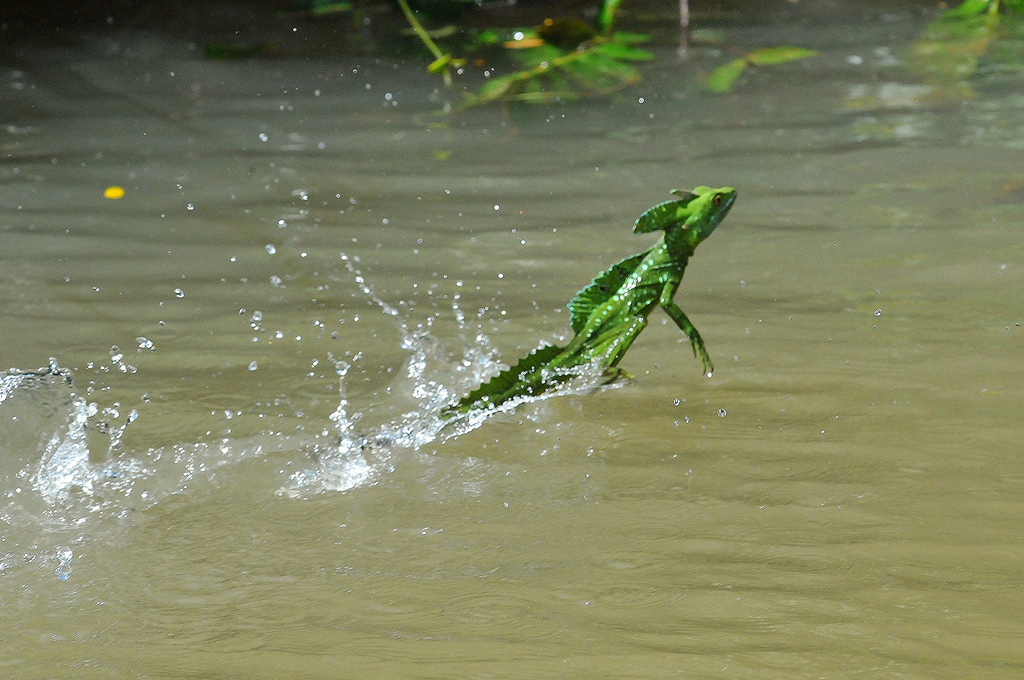
\includegraphics[width=\linewidth,height=\textheight,keepaspectratio]{water.jpg}
 
 Except maybe shallow water
=======
  Bayesian approach cannot solve experimental design issue, e.g. wanting to find effect of competition with N=2 ...
>>>>>>> b7c91fceb064dc1833fea4c4786c72d64aeb7a5a
  
 \end{frame}
 
 \begin{frame}
  \frametitle{\bf There is no bayesian model}
  
  \begin{figure}
    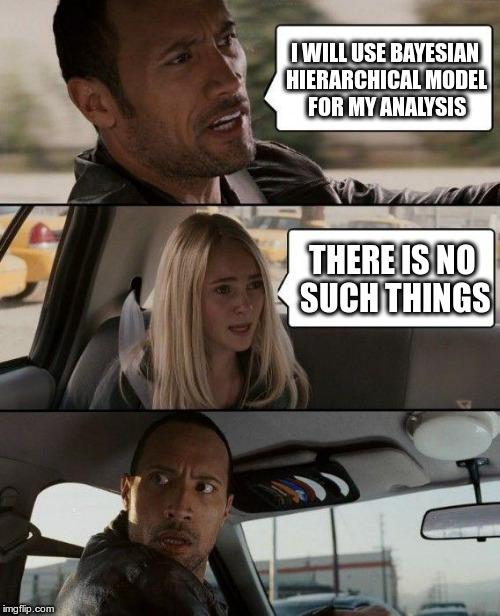
\includegraphics[width=\textwidth,height=.8\textheight,keepaspectratio]{bayes_model.jpg}
  \end{figure}

 
  

   \note{Bayesian data analaysis uses the same models as developed in classical stats,
   so there is no hierarchical bayesian models, but rather hierarchical models fit using a
   bayesian framework, this is pretty conforting as this means that we can continue fitting the same
   model we've been using except this time with all advantages confered by bayesian data analysis.}

  
 \end{frame}
 
 \begin{frame}
  \frametitle{\bf The Likelihood: what we've been doing all of our lives}
  
 \[
  lm(y \sim x1 + x2, data)
 \]

  
  This is equivalent to:
  
  \[
   y_i \sim \mathcal{N}(\mu_i,\, \sigma)   
   \]
   
   \[
    \mu_i = a + b_1 * x1 + b_2 * x2
   \]

Which is called the \textsc{likelihood}, the probability of the data given the model. 
   
  
  \note{Prob of the data knowing the parameters, what is hidden behind the (G)LM(M) motor
  
  Some plot of what this means  
  
  Good news is: we do not need to learn new models}
  
 \end{frame}
 
 \begin{frame}
  \frametitle{The likelihood: a graphical example}
  
  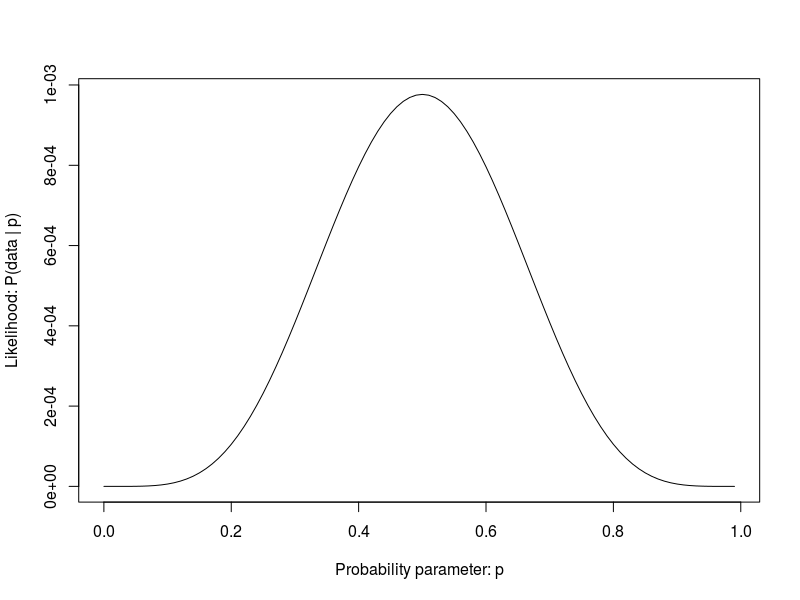
\includegraphics[width=\textwidth,height=.75\textheight,keepaspectratio]{likelihood.png}
  
  \[
   y \sim \mathcal{B}(n = 10,size = 1,prob = 0.5)
  \]
  
  \note{critical part of modelling: as long as we can write down the likelihood of our model we have great freedom}

  
 \end{frame}

 
 \begin{frame}
  \frametitle{\bf Where BDA starts}
  
  $Posterior \propto Likelihood * Prior$
  
  Or:
  
  $New knowledge \propto Current evidence * prior knowledge$
  
  Some graphical example of this
  
 \end{frame}

   \begin{frame}
  \frametitle{\bf What is prior infos}
  
  This is something new, prior is also a probability distribution that represent our beliefs of the likely values of the parameters
  This is the information that is around in the literature or in the community before doing an analysis
  Example: want to explore plant growth or whatever with a meta-analysis
  And/or information based on the nature of the parameter
  Example: a time parameter will likely be >= 0
  
 \end{frame}
 
  \begin{frame}
  \frametitle{\bf What is Posterior}
  
  The posterior is also a probability distribution, it quantifies the probability of parameter values knowing the data (the likelihood) and our expectation (prior)
  The impact of the data vs the expectation depends on the sample size, with low sample size the prior is relatively more important (little information in the data), as
  sample size grows the likelihood gets more and more weights, a simple example (maybe a shiny app ...)
  % I like the idea of the shiny app, maybe using a simple example like the prop water/land in the StatRethinking book?
  
  \end{frame}


 
 
\begin{frame}
 \frametitle{\bf The key aspects of BDA}
 
 Explicitly integrate prior knowledge 
 Output probability for the parameters/hypothesis, posterior
 Uncertainty is everywhere
 Think of models as data-generating processes
 
\end{frame}

\section{How?}

 \begin{frame}
  \frametitle{\bf Ways to fit bayesian models in R}
  
  Coding in probability language vs using wrappers
  STAN is a programming language in its own so can code the models direclty in it (some snippet code example of simple model)
  Knowing this we have the full flexibility to fit any model we want but we also have the full possibility that we make coding/interpretation
  errors that are not visible.
  There are a couple of R packages to transcribe the standard R formula synthax into STAN models: rstanarm and brms. With this option we are sure that the model
  code is correct and also optimized so it will certainly run faster than naive implementation directly in STAN. But one is limited by what the package developers have
  implemented. 
  
 \end{frame}

  \begin{frame}
  \frametitle{\bf The sampling}
  
  Blind man in the likelihood landscape, how do we effectively sample it
  
 \end{frame}
 
 \begin{frame}
  \frametitle{\bf About MCMC}
  
  Markov Chain Monte Carlo: stochastic transition within parameter space only based on current and proposed jump.
  
 \end{frame}


  \begin{frame}
  \frametitle{\bf Different samplers}
  
  JAGS: Adaptively tries to find the best sampler corresponding to your model
  STAN: Use Hamiltonian Monte Carlo (see Monnahan et al 2017 MEE)
  
 \end{frame}
 
   
  \begin{frame}
  \frametitle{\bf Elements of Bayesian vocabulary}
  
  Chains, convergence, divergence, Rhat, n\_eff
  
 \end{frame}
 
  \begin{frame}
  \frametitle{\bf Model checking in Bayesian data analysis}
  
  convergence, n\_eff, chains, posterior predictive checks
  
 \end{frame}
 
  \begin{frame}
  \frametitle{\bf Model comparison/selection}
  
  LOOC, WAIC
  
 \end{frame}
 

\section{Why?}
 
  \begin{frame}
  \frametitle{\bf Embracing uncertainty}
  
  Everything is variable, all parameters come with (posterior) distribution, can interprete posterior sample
  as probabilities, flexibility to test any hypothesis building on these
  
 \end{frame}
 
  \begin{frame}
  \frametitle{\bf Flexibility in model building}
  
  As long as you can write your likelihood function you can fit any model you like (similar to using MLE approach
  ie with bbmle)
  
 \end{frame}
 
  \begin{frame}
  \frametitle{\bf Why do we do stats?}
  
  Bayesian data analysis give us relevant answers in terms of probability rather than weird answers refering to some null hypothesis in
  terms of frequency
  
 \end{frame}
 
  \begin{frame}
  \frametitle{\bf No degrees of freedom}
  
  Fit complex models even with little data (is this something we want??)
  
 \end{frame}
 
  \begin{frame}
  \frametitle{\bf Asymptotic convergence, when bayesian and frequentist approach give similar answers}
  
  With infinite sample size the posterior distribution just reflect the likelihood, as sample size increases
  priors have dwindling effects
  
 \end{frame}
 
\end{document}


 \begin{frame}
  \frametitle{\bf }
  
 \end{frame}

